\documentclass[border=6pt]{standalone}
\usepackage{tikz}
\usetikzlibrary{arrows.meta,positioning,calc,shapes.geometric,fit,backgrounds,patterns,matrix,decorations.pathreplacing}
\begin{document}
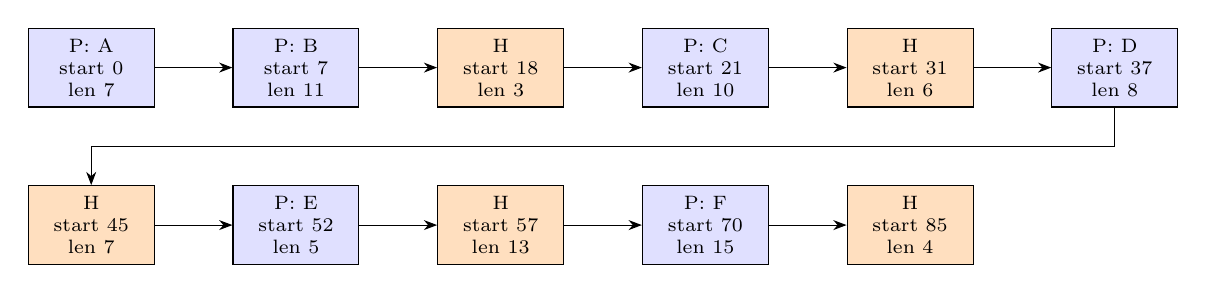
\begin{tikzpicture}[>=Stealth,font=\small]
\tikzstyle{proc}=[draw,minimum width=1.6cm,minimum height=1.0cm,align=center,font=\scriptsize,fill=blue!12]
\tikzstyle{hole}=[draw,minimum width=1.6cm,minimum height=1.0cm,align=center,font=\scriptsize,fill=orange!25]
\foreach \st/\nm/\s/\l [count=\i from 0] in {proc/P: A/0/7, proc/P: B/7/11, hole/H/18/3, proc/P: C/21/10, hole/H/31/6, proc/P: D/37/8, hole/H/45/7, proc/P: E/52/5, hole/H/57/13, proc/P: F/70/15, hole/H/85/4} {
  \pgfmathsetmacro\xx{mod(\i,6)*2.6}
  \pgfmathsetmacro\yy{-floor(\i/6)*2.0}
  \node[\st] (n\i) at (\xx,\yy) {\nm\\ start \s\\ len \l};
}
\foreach \i in {0,...,9} {\pgfmathtruncatemacro\j{\i+1} \ifnum\i=5 \else \draw[->] (n\i.east) -- (n\j.west); \fi}
\draw[->] (n5.south) -- ++(0,-0.5) -| (n6.north);
\end{tikzpicture}
\end{document}
